%!TEX root = Thesis.tex
\chapter{Implementation and Evaluation}
	The chapter contains practical part of the work, describing implementation of suggested prototype in the section
	2.3. The prototype implements the major aspects proposed in the concept (chapter 4).
	The implementation consists the major aspects proposed in the concept, according to 3-tier architecture. Namely next components:
	 \begin{itemize}
		\item \textbf{Client Tier} presents adaptive to different screens GUI, dynamically changed content and multi-user access
		\item \textbf{Application Tier} consists Apache Web-server, XMPP server and guarantee appropriate interface of collaboration between tiers via JSON format and defined structure
		\item \textbf{Data Tier} consists cookies for authorization
	\end{itemize}
	To make evaluations real, system will use data from the VICCI(Visual and Interactive Cyber-physical Systems Control and Integration) project at the Faculty of Computer Science of the Dresden University of Technology. The scope includes smart home environments and supporting people in the ambient assisted living. Also it was connected by using Data Hub as a Proxy, that is the part of Master Thesis of Luiz Alberto Borges, "Data Hub for Adaptive Data Services".
%%%%%%%%%%%%%%%%%%%%%%%%%%%%%%%%%%%
\section{Development Environment}
	As a programming languages for implementation of this work jQuery\footnote{jQuery programming language, \url{http://jquery.com/}} and HTML5\footnote{HTML specification, \url{http://www.w3.org/wiki/HTML/Specifications}} together with CSS3\footnote{CSS specification, \url{http://www.w3.org/Style/CSS/specs.en.html}} are chosen. jQuery is a fast, small, well documented, easy and widely used and feature-rich JavaScript library. In addition it has such an important properties as: chaining, easy-to-use AJAX, event handlers, CSS selectors, pluins. It makes things like HTML document traversal and manipulation, event handling, animation, and Ajax much simpler with an easy-to-use API that works across a multitude of browsers. It enables the project code to be portable over different platforms and provides opportunity for robust and effective development. The choice is dictated mostly by two aspects. On the one hand, the system that is being developed is distributed by it’s nature. On the other hand, jQuery has low entry barrier, and the code written in this language is extremely readable, laconic and understandable. These facts make further support of written code much easier for other developers that have an experience with any other JavaScript library. 
	\newline
	To show justification of choosen approach was made comprehensive comparison between main web toolkits/libraries as Dojo\footnote{Dojo documentation, \url{http://dojotoolkit.org/features/}}, Prototype\footnote{Prototype documentation, \url{http://prototypejs.org/}}, Yahoo User Interface(YUI) and ExtJS\footnote{ExtJS documentation,\url{http://docs.sencha.com/extjs/4.2.2/}} that shown in the Table 5.1. 
	\begin{table}[H]
	\centering
	\begin{tabular}{|L{3cm}|l|L{2cm}|l|L{2cm}|L{2cm}|}
	\hline
	Target 			& jQuery & Dojo & Prototype & YUI & ExtJS \\
	\hline
	\hline
	License		& MIT & BSD \& AFL & MIT & BSD & GPL and Commercial \\
	\hline
	Size		& 32 KiB & 41 kB & 46–278 kB & 31 kB & 84–502 kB \\
	\hline
	Source language		& JavaScript & JavaScript + HTML & JavaScript &  Javascript + HTML + CSS & JavaScript \\
	\hline
	Grid		& yes & yes & yes & - & yes  \\
	\hline
	DOM wrapped		& yes & yes & yes & no & yes \\
	\hline
	Other data retrieval		& XML, HTML & XML, HTML, CSV, ATOM & - & yes & XML  \\
	\hline
	DOM wrapped		& yes & yes & yes & no & yes \\
	\hline
	Server push data retrieval		& yes & yes & - & via Plugin & yes \\
	\hline
	GUI page layout		& with Plugin & yes & yes & - & yes \\
	\hline 		
	Touch events		& with Plugin & yes & yes & - & yes \\
	\hline 
	\end{tabular}
	\caption[Caption in TOC]{Comparison of JavaScript frameworks}
	\label{tab:JS_frameworks}
	\end{table}
	Also the most important part is a version of browser support. jQuery\footnote{jQuery browser support, \url{http://jquery.com/browser-support/}}, Dojo\footnote{Dojo browser support,\url{http://livedocs.dojotoolkit.org/releasenotes/1.4}}, Prototype\footnote{Prototype browser support, \url{http://prototypejs.org/doc/latest/Prototype/Browser/index.html}} , YUI\footnote{YUI browser support, \url{http://yuilibrary.com/yui/environments/}}, ExtJS\footnote{ExtJS browser support, \url{http://www.sencha.com/products/extjs/}}

	\begin{table}[H]
	\centering
	\begin{tabular}{|r|l|l|l|l|l|}
	\hline
	Target 			& jQuery & Dojo & Prototype & YUI & ExtJS \\
	\hline
	\hline
	Chrome		& 1+ & 3 & 1+ & - & 10+ \\
	\hline
	Opera		& 9+ & 10.50+ & 9.25+ & 10.0+ & 11+ \\
	\hline
	Safari		& 3+ & 4 & 2.0.4+ & 4.0 & 4+ \\
	\hline
	Mozilla Firefox		& 2+ & 3+ & 1.5+ & 3+ & 3.6+ \\
	\hline
	Internet Explorer		& 6+ & 6+ & 6+ & 6+ & 6+ \\
	\hline
	\end{tabular}
	\caption[Caption in TOC]{Browser Support}
	\label{tab:internal_results}
	\end{table}


\section{Web-based Framework Analysis}
 \begin{itemize}
	\item \textbf{Bootstrap}
	\newline
	Bootstrap is the most popular and widely used framework, nowadays. It’s a beautiful, intuitive and powerful web design kit for creating cross browser, consistent and good looking interfaces. It offers many of the popular UI components with a plain-yet-elegant style, a grid system and JavaScript plugins for common scenarios.

	It consists of four main parts:
	Scaffolding – global styles, responsive 12-column grids and layouts. Bear in mind that Bootstrap doesn’t include responsive features by default. If design needs to be responsive this functionality have to be done manually. Base CSS – this includes fundamental HTML elements like tables, forms, buttons, and images, styled and enhanced with extensible classes. Components – collection of reusable components like dropdowns, button groups, navigation controls (tabs, pills, lists, breadcrumbs, pagination), thumbnails, progress bars, media objects, and more. JavaScript – jQuery plugins which bring the above components to life, plus transitions, modals, tool tips, popovers, scrollspy (for automatically updating nav targets based on scroll position), carousel, typeahead (a fast and fully-featured autocomplete library), affix navigation, and more.
	\item \textbf{Foundation}
	\newline
	Foundation is a powerful, feature-rich, responsive front-end framework. With Foundation user can quickly prototype and build websites or apps that work on any kind of device, with tons of included layout constructs, elements and best practices. It’s built with mobile first in mind, utilitizes semantic features, and uses Zepto instead of jQuery in order to brings better user experience and faster performance.
	\newline
	Foundation has a 12-column flexible, nestable grid powerful enough to create rapidly multi-device layouts. In terms of features it provides many. There are styles for typography, buttons, forms, and various navigation controls. Many useful CSS components are provided like panels, pricing tables, progress bars, tables, thumbnails, and flex video that can scale properly your video on any device. And, of course, JavaScript plugins including dropdowns, joyride (a simple and easy website tour), Magellan ( a sticky navigation that indicates where is the user on the page), orbit (a responsive image slider with touch support), reveal (for creating modal dialogues or pop-up windows),  sections (a powerful replacement for traditional accordions and tabs), and tooltips.
	\item \textbf{GroundworkCSS}
	\newline
	GroundworkCSS is a new, fresh addition to the front-end frameworks family. It’s a fully responsive HTML5, CSS and JavaScript toolkit built with the power of Sass and Compass which gives the ability to rapidly prototype and build websites and apps that work on virtually any device.

	It offers an extremely flexible, nestable, fraction-based, fluid grid system that makes creating any layout possible. GroundworkCSS has some really expressive features like tablets and mobile grids which maintain the grid column structure instead of collapsing the grid columns into individual rows when the viewport is below 768 or 480 pixels wide. Another cool feature is a jQuery ResponsiveText plugin which allows to have dynamically sized text that adapts to the width of the viewport: extremely useful for scalable headlines and building responsive tables.
	The framework includes a rich set of UI components like tabs, responsive data tables, buttons, forms, responsive navigation controls, tiles (a beautiful alternative to radio buttons and other boring standard form elements), tooltips, modals, Cycle2(a powerful, responsive content slider), and many more useful elements and helpers. It also offers a nice set of vector social icons and a full suite of pictographic icons included in FontAwesome. To see the framework in action user can use the resizer at the top center of the browser window. This way user can test the responsiveness of the components against different sizes and viewports while exploring the framework’s features. GroundworkCSS is very well documented with many examples, and to get user started quickly the framework also provides several responsive templates. The only thing as a weakness is the missing of a way to customize download.

	\item \textbf{Gumby}            
	\newline
	Gumby is simple, flexible, and robust front-end framework built with Sass and Compass.

	Its fluid-fixed layout self-optimizes the content for desktop and mobile resolutions. It support multiple types of grids, including nested ones, with different column variations. Gumby has two PSD templates that get user started designing on 12 and 16 column grid systems.
	The framework offers feature-rich UI Kit which includes buttons, forms, mobile navigation, tabs, skip links, toggles and switches, drawers, responsive images, retina images, and more. Following the latest design trends the UI elements have Metro style flat design but can use Pretty style with gradient design too, or to mix up both styles. An awesome set of responsive, resolution independent Entypo icons, is completely integrated into the Gumby Framework. Gumby has also a very good customizer with color pickers which helps to build your custom download with ease.
	\item \textbf{Kube}
	\newline
	Lastly, if user need a solid, yet simple base without needless complexity and extras, for your new project, Kube can be the right choice. Kube is a minimal, responsive and adaptive framework with no imposed styling which gives to user the freedom to create. It offers basic styles for grids, forms, typography, tables, buttons, navigation, and other stuff like links or images.

	The framework contains one compact CSS file for building responsive layouts with ease and two JS files for implementing tabs and buttons in your designs. If user is looking for maximum flexibility and customization, user can download developer version which includes LESS files, with variables, mixins and modules.
	\end{itemize}

\begin{figure}[!ht]
\centering
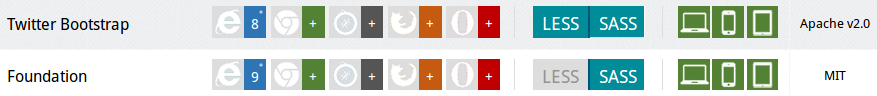
\includegraphics[scale=0.7]{images/Bootstrap&Foundation.png}
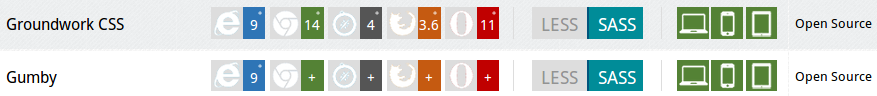
\includegraphics[scale=0.7]{images/Groundwork&Gumby.png} 

\includegraphics[scale=0.7]{images/Kube.png}  
\caption[Framework Comparison]{Framework Comparison\footnote{\url{http://usablica.github.io/front-end-frameworks/compare.html}}}
\label{img:Bootstrap&Foundation.png}
\label{img:Groundwork&Gumby.png}   
\label{img:Kube.png}                          
\end{figure}

\section{PubSub}
Data Flow model describes the 
    \begin{figure}[!ht]
    \centering
    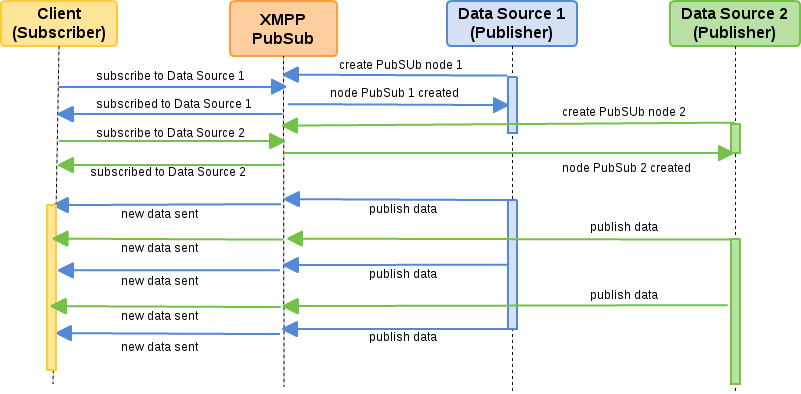
\includegraphics[scale=0.6]{images/PubSub.png}   
    \caption[Service PubSub]{Service PubSub}
    \label{img:pub_sub}                           
    \end{figure}

	\subsection{XMPP implementation}

	\subsubsection{XMPP Stanzas}
	Work is accomplished in XMPP by the sending and receiving of XMPP stanzas over an XMPP stream. Three basic stanzas make up the core XMPP toolset. These stanzas are <presence> , <message> , and <iq> . Each type of stanza has its place and purpose, and by composing the right kinds of quantities of these stanzas, sophisticated behaviors can be achieved. Remember that an XMPP stream is a set of two XML documents, one for each direction of communication. These documents have a root <stream:stream> element. The children of this <stream:stream> element consist of routable stanzas and stream related top-level children. Each stanza is an XML element, including its children. The end points of XMPP communication process input and generate output on a stanza-by-stanza basis.The following example shows a simplified and short XMPP session::
		\begin{figure}[!ht]
		\centering
		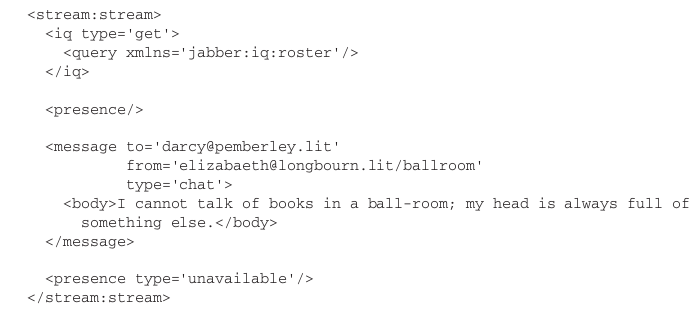
\includegraphics[scale=0.9]{images/Stanzas.png}   
		\caption[Stanzas example]{Stanzas example}
		\label{img:interfaces}                           
		\end{figure}
		In this example, Elizabeth created an XMPP stream by sending the opening <stream:stream> tag. With the stream open, she sent her first stanza, an <iq> element. This <iq> element requested Elizabeth’s roster, the list of all her stored contacts. Next, she notified the server that she was online and available with a <presence> stanza. After noticing that Mr. Darcy was online, she sent him a short <message> stanza, thwarting his attempt at small talk. Finally, Elizabeth sent another <presence> stanza to inform the server she was unavailable and closed the <stream:stream> element, ending the session.
    
    \subsubsection{Server}
	The set of XMPP servers that can mutually communicate forms an XMPP network. The set of public XMPP servers forms the global, federated XMPP network. If a server does not speak the server-to-server protocol, it becomes an island, unable to communicate with external servers. An XMPP server will usually allow users to connect to it. It is, however, also possible to write applications or services that speak the server-to-server protocol directly in order to improve efficiency by eliminating routing overhead. Anyone can run an XMPP server, and full-featured servers are available for nearly every platform. Ejabberd, Openfire, and Tigase are three popular open source choices that will work on Windows, Mac OS X, or Linux systems. Several commercial XMPP servers are available as well, including M-Link and Jabber XCP.
	
	\subsubsection{Connection}
	Before any stanzas are sent, an XMPP stream is necessary. Before an XMPP stream can exist, a connection must be made to an XMPP server. XMPP includes some sophisticated support for establishing connections to the right servers. Typically clients and servers utilize the domain name system (DNS) to resolve a server’s domain name into an address they can connect to. Email services in particular use mail exchange (MX) records to provide a list of servers that handle mail for a given domain so that one well-known server address does not have to handle every service. Email, being an early Internet application, got special treatment in DNS. These days, service records (SRV) are used to provide a similar function for arbitrary services. The first thing an XMPP client or server does when connecting to another XMPP server is to query the appropriate SRV record at the server’s domain. The response may include multiple SRV records, which can be used to load balance connections across multiple servers. If an appropriate SRV record cannot be found, the application tries to connect to the given domain directly as a fallback. Most libraries also allow you to specify a server to connect explicitly.
	\subsubsection{Long Polling}
	Even with AJAX, data was still being requested, or polled, at timed intervals. Servers can be crippled if too many clients poll too fast.However, to get quick updates, the polling interval needs to be quite small; the lowest latency possible is the length of the polling interval. Another issue with polling is that most poll requests do not receive new data. In order to see changes within a reasonable time frame of when they occur, the polling interval must be quite short, but the actual data may not change very often.
	For example, if there is new data ready on the server, the server answers immediately. If there is not new data, the server keeps the connection open, holding any reply. Once new data arrives, it finally responds to the request. If no new data arrives after some period of time, the server can send back an empty reply, so as not to hold too many open connections at once. Once a request is returned, the client immediately sends a new one, and the whole process starts over. Because each polling request is potentially open for a long period of time, this technique is called long polling. It has many advantages over normal polling.

\section{Browser Support}
	In past years a Flash-based media player in more than sufficient for streaming on the Web and this technology is still necessary to support legacy browsers. But thankfully modern standards have advanced and the inclusion of HTML5 video opens doors for dozens of new opportunities.

	In this guide I’d like to offer an introduction to HTML5 video for the Web. It will take some practice to understand the native in-browser player and all its functionality. When you’re working with a flash video player it’s all too common to associate all video formats in .flv. While this does work, most flv files cannot retain quality anywhere near the more advanced file formats/codecs. There are 3 important video types which are supported by HTML5: MP4, WebM, and Ogg/Ogv. The MPEG-4 file type is generally encoded in H.264 which allows for playback in third party Flash players. This means you don’t need to keep a .flv video copy to support a fallback method! WebM and Ogg are two much newer file types related to HTML5 video. Ogg uses Theora encoding which is based on the open-source standard audio file format. These can be saved with a .ogg or .ogv extension.
	So which of these file types do you need for your website? Well ideally all 3 would be great as they provide the full support spectrum. Yet this isn’t realistic, and in fact, you can cover all the bases with only two of them. Here is a breakdown of what works for each browser:

	Mozilla Firefox – WebM, Ogg
	Google Chrome – WebM, Ogg
	Opera – WebM, Ogg
	Safari – MP4
	Internet Explorer 9 – MP4
	Internet Explorer 6-8 – No HTML5, Flash Only!
	Most flash video players will support MP4 files as long as they’re encoded in H.264. As such, each of these browsers will embed MP4+Flash as a final resort. This means you only need to create two different video formats to support all browsers. MP4 for Safari/IE9 and a choice between WebM or Ogg for the rest.

\section{Database Model}

\section{Use Cases}

  \subsection{Frontend}
  \textbf{MVC pattern Implementation}
  Based on AngularJS

  Once an application is bootstrapped, it will then wait for incoming browser events (such as mouse click, key press or incoming HTTP response) that might change the model. Once such an event occurs, Angular detects if it caused any model changes and if changes are found, Angular will reflect them in the view by updating all of the affected bindings.

  \textbf{files in my working directory}
Most of the files in your working directory come from the angular-seed project which is typically used to bootstrap new Angular projects. The seed project includes the latest Angular libraries, test libraries, scripts and a simple example app, all pre-configured for developing a typical web app.
There are many ways to structure the code for an application. For Angular apps, was encouraged the use of the Model-View-Controller (MVC) design pattern to decouple the code and to separate concerns. 

Added Bootstrap files to app/css/ and app/img/
  \subsection{3-tier Architecture in Software Projection}
  \subsection{Use Cases Realization}
  \subsection{Evaluation}


\subsection{Summary}